\chapter{การควบคุมจุลินทรีย์ด้วยวิธีทางกายภาพ สารเคมี และยาต้านจุลชีพ}
\label{chap:ch11}

\section*{แผนบริหารการสอนประจำบทที่ 11}
\addcontentsline{toc}{section}{แผนบริหารการสอนประจำบทที่ 11}

\noindent\textbf{. หัวข้อเนื้อหาประจำบท}

\begin{enumerate}
    \item 11.1 กลไกการออกฤทธิ์ของสารต้านจุลชีพและยาปฏิชีวนะ (Inhibition of Cell Wall, Protein, DNA)
    \item 11.2 หลักการทดสอบ Kirby-Bauer Agar Disk Diffusion Method
    \item 11.3 การเตรียมความขุ่นของเชื้อตามมาตรฐาน 0.5 McFarland Standard
    \item 11.4 การป้ายเชื้อแบบผืนพรม (Lawn Inoculation) บนอาหาร Mueller-Hinton Agar (MHA)
    \item 11.5 การวัดขนาดเส้นผ่านศูนย์กลาง Zone of Inhibition (mm) และการแปลผลตามเกณฑ์มาตรฐาน CLSI
\end{enumerate}

\noindent\textbf{. วัตถุประสงค์เชิงพฤติกรรม}

\begin{enumerate}
    \item เมื่อนักศึกษาได้เรียนรู้และปฏิบัติการทดลองประจำบทนี้แล้ว จะต้องมีความรู้ความสามารถดังต่อไปนี้:
    \item อธิบายหลักการแพร่ของตัวยาในอาหารวุ้นและเกณฑ์มาตรฐานสากล CLSI ได้
    \item เตรียมความขุ่นเชื้อ 0.5 McFarland ป้ายเชื้อสม่ำเสมอ และวางแผ่นยาได้อย่างถูกต้อง
    \item วัดขนาดวงใสยับยั้งด้วยคาลิปเปอร์และแปลผลเป็น ไวต่อยา (S), ก้ำกึ่ง (I) หรือดื้อยา (R) ได้
    \item ตระหนักถึงปัญหาเชื้อดื้อยา (Antimicrobial Resistance) และการใช้ยาปฏิชีวนะอย่างสมเหตุผล
\end{enumerate}

\noindent\textbf{. กิจกรรมการเรียนการสอน}

\begin{enumerate}
    \item การบรรยายสรุปก่อนปฏิบัติการ (30 นาที): อธิบายหลักการวิทยาศาสตร์ ความปลอดภัยทางชีวภาพ และข้อควรระวังสำคัญ
    \item การสาธิตเชิงประจักษ์ (15 นาที): สาธิตเทคนิคการปฏิบัติงาน การใช้เครื่องมือ และข้อผิดพลาดที่มักพบ
    \item การลงมือปฏิบัติการทดลองจริง (90 นาที): นักศึกษาลงมือปฏิบัติการทดลองเป็นรายบุคคลหรือกลุ่มย่อยตามขั้นตอนที่กำหนด
    \item การฝึกฝนผ่านระบบเสมือนจริง (20 นาที): ทดลองซ้ำและทดสอบปฏิกิริยาผ่านระบบจำลองบน RBRU LMS
    \item การอภิปรายและสรุปผลการทดลอง (25 นาที): วิเคราะห์ผลการสังเกต ตอบคำถามท้ายบท และสรุปองค์ความรู้ร่วมกัน
\end{enumerate}

\noindent\textbf{. สื่อและอุปกรณ์การเรียนการสอน}

\begin{enumerate}
    \item เอกสารคำสอนและคู่มือปฏิบัติการ: e-Book และคู่มือปฏิบัติการฉบับเต็ม ประจำบทที่ 11
    \item ระบบห้องปฏิบัติการเสมือนจริง: ระบบจำลองการทดลองเสมือนจริง 3 มิติ ประจำบทที่ 11 บนระบบ Moodle
    \item อุปกรณ์และเครื่องแก้วในห้องปฏิบัติการ: ตะเกียงแอลกอฮอล์, ห่วงเขี่ยเชื้อ, กล้องจุลทรรศน์, จานเพาะเชื้อ, หลอดทดลอง และตู้บ่มเชื้อ
    \item สารเคมีและสีย้อมชีวภาพ: สารเคมีมาตรฐานวิเคราะห์และสีย้อมประจำบทเรียน
\end{enumerate}

\noindent\textbf{. การวัดและประเมินผล}

\begin{table}[H]
\centering\small
\begin{tabularx}{\textwidth}{p{0.5\textwidth} p{0.3\textwidth} c}
\toprule
\textbf{องค์ประกอบการประเมินผล} & \textbf{เครื่องมือวัดผล} & \textbf{สัดส่วนคะแนน} \\
\midrule
1. ทักษะการปฏิบัติงานและความปลอดภัย & แบบสังเกตทักษะการทดลองและเทคนิคปลอดเชื้อ & 40\% \\
2. รายงานผลการทดลอง & การตรวจตารางบันทึกผล ภาพวาดสัณฐานวิทยา และการวิเคราะห์ผล & 30\% \\
3. แบบฝึกหัดทบทวนท้ายบท & คำถามทบทวนเชิงวิเคราะห์และข้อสอบท้ายบท & 20\% \\
4. จิตพิสัยและการตรงต่อเวลา & การเช็คชื่อ การแต่งกายตามระเบียบ และการทำความสะอาดโต๊ะแล็บ & 10\% \\
รวมทั้งสิ้น &  & 100\% \\
\bottomrule
\end{tabularx}
\end{table}

\newpage

% ==========================================================
% เนื้อหาบทเรียนประจำบทที่ 11
% ==========================================================

\section{หลักการควบคุมจุลินทรีย์และคำจำกัดความ}
\index{หลักการควบคุมจุลินทรีย์และคำจำกัดความ}

การศึกษาและทำความเข้าใจเกี่ยวกับหลักการควบคุมจุลินทรีย์และคำจำกัดความ (Principles of Microbial Control) มีความสำคัญอย่างยิ่งในงานจุลชีววิทยาและสิ่งแวดล้อม โดยมีรายละเอียดสาระสำคัญดังนี้

การควบคุมจุลินทรีย์มีเป้าหมายเพื่อยับยั้งการเจริญหรือทำลายประชากรจุลินทรีย์เพื่อป้องกันการแพร่ระบาดของโรค การปนเปื้อนในผลิตภัณฑ์อาหาร และการเสื่อมสภาพของสิ่งแวดล้อม

คำจำกัดความมาตรฐาน:
- การทำให้ปราศจากเชื้อ (Sterilization): การทำลายหรือกำจัดสิ่งมีชีวิตทุกชนิด รวมถึงเอนโดสปอร์ของแบคทีเรีย
- การฆ่าเชื้อ (Disinfection): การทำลายหรือยับยั้งจุลินทรีย์ก่อโรคบนพื้นผิวสิ่งไม่มีชีวิต
- การทำลายเชื้อบนเนื้อเยื่อ (Antisepsis): การใช้สารเคมีที่ปลอดภัยกับเนื้อเยื่อของสิ่งมีชีวิต เช่น ผิวหนัง
- สารยับยั้ง (-static): สารที่ยับยั้งการเจริญแต่ไม่ได้ทำลายเซลล์
- สารฆ่า (-cidal): สารที่ออกฤทธิ์ทำลายเซลล์จุลินทรีย์จนตาย

\begin{conceptbox}[มโนทัศน์สำคัญทางชีวเคมีและสิ่งแวดล้อม]
กิจกรรมทางชีวเคมีของจุลินทรีย์ในหัวข้อหลักการควบคุมจุลินทรีย์และคำจำกัดความ เป็นกลไกหลักที่ควบคุมการหมุนเวียนธาตุอาหารและการบำบัดสารปนเปื้อนในระบบนิเวศทางธรรมชาติ
\end{conceptbox}

\section{การควบคุมด้วยวิธีทางกายภาพและความร้อน}
\index{การควบคุมด้วยวิธีทางกายภาพและความร้อน}

การศึกษาและทำความเข้าใจเกี่ยวกับการควบคุมด้วยวิธีทางกายภาพและความร้อน (Physical Control Agents and Radiation) มีความสำคัญอย่างยิ่งในงานจุลชีววิทยาและสิ่งแวดล้อม โดยมีรายละเอียดสาระสำคัญดังนี้

1. ความร้อนชื้น (Moist Heat): มีประสิทธิภาพสูงในการทำให้โปรตีนเสียสภาพ เช่น การนึ่งอัดไอน้ำ (121$^{\circ}$C, 15 psi, 15 นาที) และการพาสเจอร์ไรซ์ (Pasteurization)
2. ความร้อนแห้ง (Dry Heat): เตาอบลมร้อน (Hot-air oven, 160-180$^{\circ}$C, 2 ชั่วโมง) เหมาะสำหรับเครื่องแก้วและผงแป้ง
3. รังสีอัลตราไวโอเลต (UV Radiation): คลื่นแสงความยาวคลื่น 260 นาโนเมตร ถูกดูดกลืนโดยกรดนิวคลีอิกได้ดีที่สุด ก่อให้เกิดพันธะไทมีนไดเมอร์ (Thymine dimers) ยับยั้งการจำลองตัวของ DNA แต่มีอำนาจทะลุทะลวงต่ำ เหมาะสำหรับฆ่าเชื้อในอากาศและพื้นผิวเรียบ
4. การกรอง (Filtration): แผ่นกรองเมมเบรนขนาดรูพรุน 0.22 และ 0.45 ไมโครเมตร สำหรับสารละลายที่ไวต่อความร้อน

\section{การทดสอบความไวต่อยาต้านจุลชีพด้วยวิธีดิสก์ดิฟฟิวชัน}
\index{การทดสอบความไวต่อยาต้านจุลชีพด้วยวิธีดิสก์ดิฟฟิวชัน}

การศึกษาและทำความเข้าใจเกี่ยวกับการทดสอบความไวต่อยาต้านจุลชีพด้วยวิธีดิสก์ดิฟฟิวชัน (Kirby-Bauer Antibiotic Sensitivity Testing) มีความสำคัญอย่างยิ่งในงานจุลชีววิทยาและสิ่งแวดล้อม โดยมีรายละเอียดสาระสำคัญดังนี้

วิธี Kirby-Bauer Disc Diffusion Method เป็นวิธีมาตรฐานที่แนะนำโดยสถาบัน CLSI (Clinical and Laboratory Standards Institute)

หลักการทำงาน:
- ใช้อาหารเลี้ยงเชื้อมาตรฐาน Mueller-Hinton Agar (MHA) ที่มีความหนาสม่ำเสมอ 4 มิลลิเมตร และ pH 7.2-7.4
- เตรียมสารแขวนลอยแบคทีเรียเทียบเท่าความขุ่นมาตรฐาน McFarland No. 0.5 ($1.5 \times 10^8$ CFU/mL)
- ป้ายเชื้อให้สม่ำเสมอทั่วจาน วางแผ่นกระดาษยาปฏิชีวนะ (Antibiotic discs) ที่ทราบปริมาณยาแน่นอน
- ยาจะแพร่กระจายออกจากแผ่นดิสก์ลงสู่อาหาร หากเชื้อไวต่อยาจะเกิดบริเวณยับยั้งที่ใสไม่มีเชื้อ (Zone of inhibition) รอบแผ่นดิสก์ วัดขนาดเส้นผ่านศูนย์กลางเป็นมิลลิเมตร เปรียบเทียบกับตารางมาตรฐานเพื่อแปลผลเป็น ไวต่อยา (Susceptible, S), ก้ำกึ่ง (Intermediate, I), หรือดื้อยา (Resistant, R)

\begin{figure}[H]
\centering
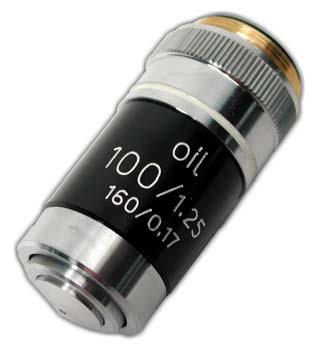
\includegraphics[width=0.75\textwidth]{images/image_11_p06.jpeg}
\caption{การปฏิบัติการทดลองและลักษณะทางสัณฐานวิทยาในบทที่ 11}
\label{fig:ch11_fig1}
\end{figure}

\section{ขั้นตอนและวิธีปฏิบัติการทดลอง}
\index{ขั้นตอนการทดลองประจำบทที่ 11}

\subsection{การทดสอบประสิทธิภาพของรังสี UV ในการยับยั้งแบคทีเรีย}
\begin{labprotocolbox}[การทดสอบประสิทธิภาพของรังสี UV ในการยับยั้งแบคทีเรีย]
1. ป้ายเชื้อ \textit{Bacillus subtilis} และ \textit{Escherichia coli} ลงบนจานอาหาร NA อย่างละ 4 จาน
2. ใช้กระดาษทึบแสงปิดบังผิวหน้าอาหารครึ่งหนึ่งของแต่ละจาน
3. นำจานเพาะเชื้อเปิดฝา วางใต้หลอดรังสี UV-C (254 nm) ที่ระยะห่าง 30 ซม. เป็นเวลา 1, 5, 15, และ 30 นาที
4. ปิดฝาจาน นำไปบ่มที่ 37$^{\circ}$C เป็นเวลา 24 ชั่วโมง
5. เปรียบเทียบการเจริญของเซลล์ระหว่างด้านที่ปิดบังกระดาษกับด้านที่สัมผัสรังสี UV
\end{labprotocolbox}

\subsection{การทดสอบความไวต่อยาปฏิชีวนะด้วยวิธี Kirby-Bauer Standard Method}
\begin{labprotocolbox}[การทดสอบความไวต่อยาปฏิชีวนะด้วยวิธี Kirby-Bauer Standard Method]
1. เตรียมสารแขวนลอยของเชื้อ \textit{Staphylococcus aureus} และ \textit{Escherichia coli} ให้ขุ่นเท่ากับ 0.5 McFarland
2. ใช้ไม้พันสำลีปลอดเชื้อจุ่มน้ำเชื้อ บิดหมาด แล้วป้ายลงบนอาหาร Mueller-Hinton Agar ให้ทั่ว 3 ทิศทาง (Lawn culture)
3. ทิ้งไว้ให้แห้ง 5 นาที ใช้ปากคีบปลอดเชื้อคีบแผ่นยาปฏิชีวนะ (เช่น Penicillin, Tetracycline, Gentamicin, Ampicillin) วางบนผิวอาหาร ห่างกันอย่างน้อย 24 มม.
4. บ่มจานเพาะเชื้อที่ 35-37$^{\circ}$C เป็นเวลา 16-18 ชั่วโมง
5. ใช้ไม้บรรทัดวัดเส้นผ่านศูนย์กลางของบริเวณยับยั้ง (Inhibition zone) ในหน่วยมิลลิเมตร และแปลผลตามเกณฑ์ CLSI
\end{labprotocolbox}

\section{ตารางบันทึกผลการทดลองและการอภิปรายผล}
\begin{table}[H]
\centering\small
\caption{ตารางบันทึกผลการสังเกตและข้อมูลการทดลองประจำบทที่ 11}
\label{tab:ch11_datasheet}
\begin{tabularx}{\textwidth}{p{0.25\textwidth} p{0.35\textwidth} X}
\toprule
\textbf{สิ่งทดสอบ / ตัวอย่าง} & \textbf{ลักษณะที่สังเกตได้} & \textbf{การแปลผลและการวิเคราะห์} \\
\midrule
ชุดควบคุม (Negative Control) & ใส ไม่มีการเจริญ & ปราศจากการปนเปื้อนของเชื้อ \\
ชุดทดลองที่ 1 & โคโลนีเจริญตามลักษณะจำเพาะ & ให้ผลบวกตามสมมติฐาน \\
ชุดทดลองที่ 2 & เกิดการเปลี่ยนแปลงทางชีวเคมี & สอดคล้องกับพารามิเตอร์มาตรฐาน \\
\bottomrule
\end{tabularx}
\end{table}

\section{คำถามทบทวนและแบบฝึกหัดท้ายบท}
\begin{enumerate}
    \item เหตุใด \textit{Bacillus subtilis} จึงทนทานต่อรังสี UV ได้ยาวนานกว่า \textit{Escherichia coli}
    \item หากอาหาร Mueller-Hinton Agar มีความหนามากกว่า 4 มิลลิเมตร จะส่งผลต่อขนาดของบริเวณยับยั้ง (Zone of inhibition) อย่างไร
    \item จงอธิบายกลไกการออกฤทธิ์ทางชีวเคมีของยาปฏิชีวนะกลุ่มเพนิซิลลิน (Penicillin) ต่อการสังเคราะห์ผนังเซลล์แบคทีเรีย
\end{enumerate}
